\documentclass[]{iat}

%Hier können weitere benötigte Pakete Eingebunden werden
%\usepackage[backend=biber,style=alphabetic,]{biblatex}
\usepackage{float}
\usepackage{listingsutf8}
\usepackage{color}
\usepackage{gensymb}
\usepackage{caption}
\usepackage{hyperref}
\usepackage{subcaption}
%Namen eingeben / Insert Name
\renewcommand{\author}{Nico Spiske}
%Art der Arbeit / Scope (Project, Thesis...)
\providecommand{\scope}{Bachelorarbeit}
%Thema der Arbeit / Theme of Thesis
\renewcommand{\subject}{Lösungsansätze für die Regelung von dynamischen Systemen mittels
Reinforcement Learning Algorithmen}
%Schlagwörter / Keywords
\providecommand{\keywords}{}
%Literaturliste *.bib / Bibliography
\providecommand{\bibfile}{literature}
%Matrikelnummer / Student ID
\providecommand{\studentID}{4436923}
%Betreuer /& Tutors
\providecommand{\tutora}{M.Sc. Ricardo Bosold}
\providecommand{\tutorb}{M.Sc. Phillipp Hendrys}
%Prüfer / Examiner
\providecommand{\examinera}{Prof. Dr.-Ing. Kai Michels}
\providecommand{\examinerb}{Dr.-Ing. Dennis Pierl}
%Farben
\definecolor{dkgreen}{rgb}{0,0.6,0}
\definecolor{gray}{rgb}{0.5,0.5,0.5}
\definecolor{mauve}{rgb}{0.58,0,0.82}
\definecolor{darkblue}{rgb}{0.0,0.0,0.6}
\definecolor{cyan}{rgb}{0.0,0.6,0.6}
%lst überschrift
\captionsetup[lstlisting]{font={Large}}

\hypersetup{%
	pdftitle	={\subject -- \author -- \today},
	pdfauthor	={\author},
	pdfsubject	={\subject},
	pdfkeywords ={\keywords}
}

\addbibresource{literature.bib}

\setlength{\footheight}{21pt}

\begin{document}
%Pfad zu Grafiken:
\graphicspath{{./project_graphics/}}
% Sprachauswahl /Language Selection (ngerman/english)
\selectlanguage{ngerman}
% \pagenumbering{roman}
\begin{titlepage}
    \newgeometry{left=0cm,right=0cm,top=0cm,bottom=0cm}
    {\color{iatred}\rule{\textwidth}{1cm}}
    \begin{minipage}{0.7\textwidth}
        \vspace{-1.37cm}
        {\color{iatred}\rule{\textwidth}{0.5cm}}
    \end{minipage}%
    \begin{minipage}{0.3\textwidth}
        \raggedright
        \vspace{0.4cm}
        \hspace{0.35cm}
        \includegraphics[scale=1]{Logos/iat_logo_en}
    \end{minipage}%
    \centering
    \vspace{4cm}
    
        {\Large
            \textbf{\scope}
        }\par
    
    \vspace{2cm}
    
        {\linespread{1.1}\huge\sffamily\bfseries
         \subject\par}
    
    \vspace{2cm}
    
        {\large
         \author\\
         \studentID
        \par}
    
    \vspace{1cm}
    
        \today
        
    \vspace{3cm}
    \begin{table}[h]
        \centering
        \begin{tabular}{lll}
            \underline{Betreuer:}	&\quad\hspace{4cm}\quad&\underline{Gutachter:}\hspace{5cm}\\
            \tutora	&	&\examinera\\
            \tutorb	&	&\examinerb
        \end{tabular}
    \end{table}
    \thispagestyle{empty}  
    \vfill
    \begin{minipage}{0.3\textwidth}
        \centering
    %	\hspace{2cm}
        \includegraphics[scale=1.2]{Logos/uni_logo_title}\relax
            \vspace{0.1cm}
    \end{minipage}%
    \begin{minipage}{0.7\textwidth}
        \raggedleft
        {\color{iatred}\rule{\textwidth}{0.5cm}}
        \vspace{-0.9cm}
    \end{minipage}
    {\color{iatred}\rule{\textwidth}{1cm}}
    \end{titlepage}
    
%Urherberrechtserklärung / Confirmation of Conformity Comment if not needed
\chapter*{Urheberrechtliche Erklärung}
Hiermit versichere ich, dass ich meine Abschlussarbeit ohne fremde Hilfe angefertigt habe und dass ich keine Anderen als die von mir angegebenen Quellen und Hilfsmittel benutzt habe.\par
Alle Stellen, die wörtlich oder sinngemä{\ss} aus Veröffentlichungen entommen sind, habe ich unter Angabe der Quellen als solche kenntlich gemacht.\par
Die Abschlussarbeit darf nach der Abgabe nicht mehr verändert werden.\par
\vspace{2.5em}
Datum:\underline{\hspace{3.5cm}}\qquad Unterschrift:\underline{\hspace{5.5cm}}
\vspace{3em}
\section*{Erklärung zur Veröffentlichung von Abschlussarbeiten}
$\Box$ Ich bin damit einverstanden, dass meine Abschlussarbeit im Universitätsarchiv für wissenschaftliche Zwecke von Dritten eingesehen werden darf.\par
$\Box$ Ich bin damit einverstanden, dass meine Abschlussarbeit nach 30 Jahren (gem. §7 Abs.2 BremArchivG) im Universitätsarchiv f`ür wissenschaftliche Zwecke von Dritten eingesehen werden darf.\par
$\Box$ Ich bin \textit{nicht} damit einverstanden, dass meine Abschlussarbeit im Universitätsarchiv für wissenschaftliche Zwecke von Dritten eingesehen werden darf.\par
\vspace{2.5em}
Datum:\underline{\hspace{3.5cm}}\qquad Unterschrift:\underline{\hspace{5.5cm}}


\tableofcontents

\newpage

\chapter{Einleitung} \label{sec:einleitung}
\section{Motivation} \label{sec:motivation}
Die dynamischen Systeme oder auch Regelstrecken, welche es heutzutage überall auf der Welt gibt, werden immer größer und komplexer. Sie finden sich als kleine einfach zu regelnde Systeme, wie ein automatische Heizung, welche durch einfaches an und ausschalten das Ziel hat abhängig von einem Therometer gelesenen Wert eine Raumtemeperatur konstant zu halten. Allerdings finden sich auch als komplexe Regelkreise wieder, wie in Fabriken oder in Kraftwerken wie das Bremer Müllheizkraftwerk wieder. Hier exisitieren auch zum Beispiel Thermometer, welche die aktuelle Temperatur eines Prozesses wiedergebene und wonach dann ein Regler sich einstellt um diesen gewollt zu verändern. Nur exisitieren hier auch viele Störgrößen, welche einen gezielten Reglerentwurf sehr schwierig machen. Störgrößen können unbekannt oder gar ungeplannt sein, so kann im Falle des Bremer Müllheizkraftwerks auf die Menge, welche zu einem Zeitpunkt verbrannt wird eingegangen werden, wie heiß die nächste Ladung an Müll jedoch brennen wird ist relativ unbekannt und stark variierend. Abhilfe für den Reglerentwurf für komplexe Regelkreise sollen Algorithmen bieten, welche selbstständig lernen können den richtigen Stelleingriff in einem gewollten System vorzunehmen.
\section{Zielsetzung} \label{sec:zielsetzung}
Das Ziel dieser Arbeit soll es sein, mittels eines Reinforcement Learning Agentens ein Beispielhaftes dynamisches Modell zu regeln. Gezeigt werden sollen außerdem Methoden um dynamische Systeme mit Hilfe von bestehenden Methodiken zu erstellen und sie anschließend mit dem Agenten zu verbinden. Die Methode um die Grundmodelle zu erstellen, soll Simulink von MatLab bieten. Der Grund hierfür ist, da bereits ein bestehendes Grundverständnis für das Toolkit exisiert und außerdem Simulink mit seinen zahlreichen Schaltblöcken eine elegante Methode anbietet, um eine Modellbildung durchzuführen. Das in Simulink erstellte Modell, soll dann anschließend in ein Python Modell transformiert werden, damit dadurch die Möglichekeit besteht die zahlreichen Bibliotheken für maschinelles Lernen zu verwenden, welche Python besitzt. Der Reinforcement Learning Agent, welcher mit dem Modell arbeiten soll und die Aufgabe hat es zu regeln, soll in Python mit den wie bereits erwähnten Bibliotheken aus dem Bereich des maschinellen Lernens implementiert werden. Als Beispielhaftes dynamisches Modell soll ein Kräftemodell für ein Schiff verwendet werden, welches durch Störgrößen wie dem Wind, oder dem treiben des Schifs beeinflusst wird. Der Agent soll die möglichkeithaben dieses Modell zu regeln indem er mit dem Schiffantrieb und seinem Ruder interagieren darf.

\section{Aufbau der Arbeit} \label{sec:aufbau_arbeit}
Damit nun das dynamische Modell erstellt und anschließend in ein Environment umgewandelt werden kann, in welchem ein Reinforcement Learning Agent existieren kann, soll zuerst geklärt werden, woher der Begriff des Reinforcement Learnings überhaupt kommt. Eine Übersicht, in worein sich der Begriff eingelieder und was genau er wirklich bedeutet, findet sich in Kapitel \ref{sec:reinforcement_learning} und seinen Unterkapiteln. In diesem Kapitel wird damit angefangen zu erläutern, was genau maschinelles Lernen überhaupt ist und wie es sich grob aufspaltet in seine drei Arten. Diese drei Arten sollen erklärt werden, damit es dem Leser möglich ist, diese von einander trennen zu können und die Wichtigkeit der Reinforcement Learning Algorithmen zu erkennen. Es soll anschließend eine Übersicht geboten werden, in welcher die verschiedenen wichtigen Reinforcement Learning Algortihmen mit einander verglichen werden. Folgend auf die Übersicht, kommt dann auch schon die Einführung zum Thema der Soft Actor-Critic (SAC) Agenten beziehungsweise Algorithmen, welche für diese Arbeit verwendet wurden zu realisierung des Modell Reglers. Vor allem der Soft Actor-Critic soll detailreicher mit tieferem Verständnis erläutert werden, damit in einem späteren Kapitel der Arbeit die Implementierung innerhalb von Python verständlich ist. Hierzu soll unteranderem durch Pseudocode die Hauptkomponenten visualisert werden zusammen mit den dazugehörenden wichtigen Konzepten.\\
Nach dem der Teil des maschinellen Lernens verdeutlicht wurde, folgen die Einblicke in die tatsächliche implementierung des Soft Actor-Critic Agenten in Python zusammen mit der PyTorch Bibliothek, welche für diese Arbeit als Framework für das maschinelle Lernen gewählt wurde. Es soll hier gezeigt werden, wie die Hauptkomponenten implementiert wurden, und wie diese dann vorab schon vor der Erläuterung des Modells in Python beziehungsweise des Environments, mit in den Schnittstellen des Environments eingebunden wurden. Anschließend folgt das Unterkapitel \ref{sec:imp_simulink}, in welchem die Modellbildung für das Schiffmodell in Simulink erläutert wird. Hierbei soll gezeigt werden, wie sich das gewählte Schiffmodell zusammensetzt und was für Kraftgleichungen aufgestellt wurden um diese zu realisieren. Damit soll dem Leser klar werden, welche Störgrößen nun exisieren, wo genau der Agent Kontrolle über das Schiff hat und wie dieses nun überhaupt im Environment später sich verhalten wird wenn dann die Simulationen anfangen. Da der Agent in Python nun zu disem Zeitpunkt bereits in Python implementiert wurde, folgt auf die Modellbildung in Simulink auch schon die Umsetzung des erstellten Modells in Python. Hierfür soll vorerst gezeigt werden Anhang eines einfacheren Modells, wie diese Umsetzung funktionieren wird. Es wird dabei auf die Implementierung der Integratoren aus Simulink innerhalb von Python eingegangen, da diese mit ein Kernstück bilden für die ganze Modellbildung und demnach unverzichtbar sind. Nach der Beispielumsetzung, folgt dann auch die tatsächliche Umsetzung des Schiffmodells in Python und wie dieses in ein Gym Environment von OpenAI eingebunden wurde, damit der Agent dann auch mit ihm interagieren kann. Als Finale werden dann die verschiedenen Ergebnisse dieser Arbeit präsentiert, zusammen mit einer Diskussion wie diese zustande kommen und einer anschließenden Zusammenfassung mit einem Ausblick wie es weiter gehen könnte in dieser Thematik.

\chapter{Reinforcement Learning} \label{sec:reinforcement_learning}
Im Zeitalter der Information, in welchem wir uns heutzutage befinden, gibt es eine unbegreiflich große und stätig wachsende Menge an Daten. Dies erkannte bereits der Trend- und Zukunftsforscher John Naisbitt im Jahre 1982 in seinem Buch Megatrends.
\begin{align*}
    \text{Wir ertrinken in Informationen, aber hungern nach Wissen. - John Naisbitt}
\end{align*}
Aufgrund dieser riesigen Menge an Daten, gibt es eine große Nachfrage nach automatisierten Methoden, um diese Daten letztendlich auch auswerten und analysieren zu können. Abhilfe für diese Nachfrage, beziehungsweise für dieses Problem soll das Teilgebiet des maschinellen Lernens aus dem Oberbegriff der künstlichen Intelligenz bieten. Das maschinelle Lernen bietet hierbei eine Facette aus verschiedenen Algorithmen und Methoden um innerhalb der untersuchten Daten das zu finden, was der Benutzer braucht. Hierbei können die Daten nach bereits bekannten Mustern untersucht werden, oder es kann nach unbekannten Mustern gesucht werden, es können auch vorhersagen getroffen werden aus dem bestehenden Datensatz umso zum Beispiel Marktforschung betreiben zu können. Wie sich das maschinelle Lernen als Oberthema nun zusammensetzt, und wo genau der Schwerpunkt dieser Arbeit, dass Reinforcement Learning sich als Begriff wieder findet, soll in diesem Kapitel verständigt werden.

\section{Maschinelles Lernen} \label{sec:machine_learning}
Das maschinelle Lernen auch Machine Learning oder kurz ML, kann im ganzen in drei Kategorien unterteilt werden. Hierbei gibt es das überwachte Lernen, unüberwachte Lernen und das bestärkte Lernen wobei letzeres dem in dieser Arbeit fokusierte Reinforcement Learning entspricht, wie es im großteil der Literatur genannt wird. Bevor die tatsächlichen Grundlagen des Reinforcement Learnings erklärt werden sollen, soll außerdem noch einmal auf die beiden anderen Algorithmenarten eingegangen werden, um für eine Übersicht und somit für ein besseres Verständnis zu sorgen.

\subsection{Überwachtes Lernen} \label{sec:ueberwachtes_lernen}
Machine Learning Konzepte welche sich innerhalb des Bereichs des Überwachten Lernens finden, sind mit an verbreitesten. Bei ihnen kann unterschieden werden zwischen Ansätzen, welche zur klassifizierung dienen und jene Ansätze welche Regressionsprobleme lösen sollen. Grundsätzlich kann gesagt werden das beide dieser Ansätze dennoch dem selben Prinzip folgen. Beim überwachten Lernen werden große Mengen an Daten verwendet um diverese ML Konzepte wie neuronale Netzwerke, Support Vector Machines oder Decision Trees zu trainieren. Die Datensätzen definieren sich dabei durch eine Abbildung von den sogenannten Features auf die Labels. Im Fall des Trainingsprozesses bekommen die Implementationen, welche auf dem Konzept des überwachten Lernens basieren, beide Seiten der Abbildung. Dies bedeutet das im Falle eines neuronalen Netzwerkes der Input Layer die Features des Datensatzes bekommen würde, während der Output Layer die zu den Feature gehörenden Labels bekommt.\\
Die bereits genannten Grundansätze beim überwachten Lernen, Regression und Klassifizierung unterscheiden sich durch zwei wesentlichen Ideen. Im Falle eines Regressionsproblems ist es das Ziel, die Abbildung zu verstehen, welche mit einem gegebenen Datensatz beim Training definiert ist. Das Ziel ist somit in vielen Fällen die Vorhersage von Datenwerten basierend auf den Labels, welche als Input gegeben werden. Dies kann zum Beispiel die Vorhersage von Hauspreisen sein, basierend auf die Grundstückfläche, dem Alter des Hauses und der Kriminalitätsrate der Umgebung wo das Haus steht sein. Bei einer Klassifizierung werden auch Datensätze verwendet, welche eine Abbildung der Features auf die Labels darstellt. Der große Unterschied zu einem Regressionsproblem besteht jedoch hierbei daraus, dass keine nicht einfach nur Werte vorhergesagt werden sollen. Stattdesen ist das Ziel bei einer Klassifizierung zum Beispiel das richtige Objekt auf einem Bild zu erkennen, oder ob eine Nachricht in einem E-Mail Posteingang Spam ist oder nicht. Der Datensatz beim Training könnte somit bei den Features eine Ansammlung an Bilder mit jeweils Orangen und Äpfeln sein, während die Labels dazu aussagen ob auf dem jeweiligen Bild eine Orange oder ein Apfel zu sehen ist.

\subsection{Unüberwachtes Lernen} \label{sec:unueberwachtes_lernen}
Konzepte aus der Kategorie des unüberwachten Lernens dienen hautpsächlich dazu die drei Aufgaben oder Probleme zu lösen, welche sich mit dem Clustering, Assoziieren und der dimensionalen Reduktion befassen. Auch für das unüberwachte Lernen werden wieder große Mengen an Datensätzen benötigt, der Unterschied zum überwachten Lernen liegt hier jedoch darin, dass das unüberwachte Lernen lediglich die Features als Input bekommt und keine dazu gehörenden Labels. Einem solchen unüberwachten Algorithmus ist somit die möglichkeit geboten die Datensätze frei zu erforschen und in ihnene zum Beispiel Muster zu erkennen. Algorithmen welche sich beim unüberachten Lernen wiederfinden sind oftmals K-Means, Gaussian Mixture Models, Principal Component Analysis (PCA) oder wieder neuronale Netzwerke.\\
Probleme aus dem Aufgabenbereich des Clusterings handeln davon, dass es Datensätze gibt, welche zum Beispiel Blumenarten beschreiben. Das verwendete Beispiel ist hierbei das \textit{Iris} Flower Dataset. Das Ziel könnte es nun sein, dass analysiert werden soll wie viele unterschiedliche Blumenarten es in diesem Datensatz wirklich gibt. Dies könnte nun dadurch geschehen, indem sich ein unüberwachter Algorithmus die 5 verschiedenen Features anschaut, welche beim Beispiel Datensatz mit gegeben wurden. Diese Features wären dann Blumeneigenschaften wie die länge und breite der Kelchblätter sowie die länge und breite der Kronblätter und die Farbe der jeweiligen Blätter. Die richtige Kombination aus länge und breite der jeweiligen Blätter zusammen mit deren Farbe könnte nun zum Beispiel 3 verschiedene Blumenarten beschreiben, welche intern somit 3 Cluster darstellen würden. Visualisert finden sich diese 3 beschriebenen Cluster für die jeweilige Blumenart nocheinmal in der folgenden Abbildung \ref{abb:flower_example}.
\begin{figure}[H]
    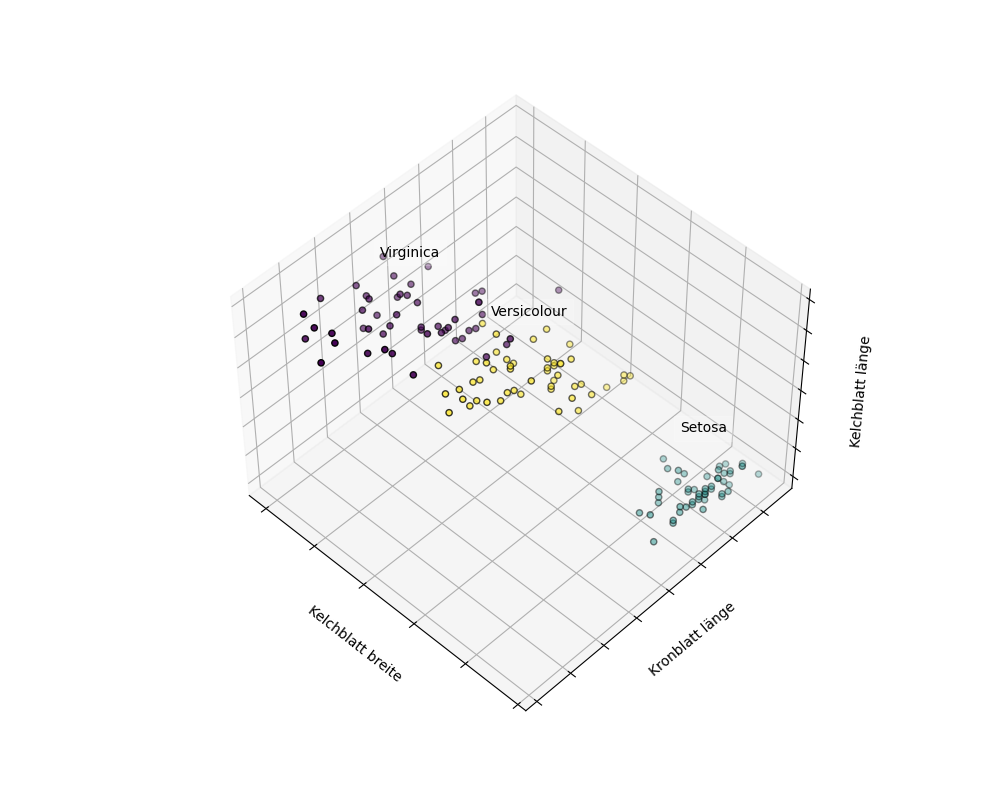
\includegraphics[width=0.9\textwidth]{graphics/iris_set_groundtruth.png}
    \centering
    \caption{Die drei beschriebenen Blumensarten aus dem Beispiel Datensatz visualisiert in ihrem jeweiligen Cluster. Verwendete Achsen sind die 3 relevantesten Features des Datensatzes für die Beschreibung einer jeweiligen Blumenart.}
    \label{abb:flower_example}
\end{figure}
Unüberwachte Algorithmen besitzen auch die Fähigkeit Assoziationen in Datensätzen zu entdecken. Hierbei können die Algorithmen innerhalb eines gewählten Datensatzes zum Beispiel noch unbekannte zusammenhänge oder Abbildungen zwischen den einzelnen Datenpunkten erkennen und herausfiltern. Solche zusammenhänge sind dann Eigenschaften wie Muster, welche alle n Datenpunkte auftauchen, oder wie zwischen mehreren Datenpunkten zusammen ein Verbindung steht und diese Einfluss auf andere Datenpunkte haben. Ein klassiches Beispiel hierfür sind Anzeigen beim Onlinekauf, in welchem Produkte gezeigt werden, welche oft zusammen mit dem gekauft wird, was der Kunde gerade betrachtet.\\
Das letzte Beispiel, die reduktion der Dimensionen wird oftmals für die anderen ML Konzepte verwendet. Vor allem bei Algorithmen, welche auf überwachten Lernen basieren kann eine solche Dimensionsreduktion helfen, da hierbei die Anzahl der Features reduziert werden kann. Eine reduzierte Anzahl an Features hat damit den Vorteil, dass die Modelle schneller und gegebenenfalls mit höherer Prezision trainiert werden können, da irrelevante Daten durch die Reduktion entfernt werden. Klassisch wird für eine solche reduktion der Principal Component Analysis oder kurz PCA Algorithmus verwendet.

Da die zuvor erwähnten neuronalen Netzwerke für die Implementierung des Agenten verwendet wurden, sollen diese noch einmal zusammengefasst erklärt werden in dem folgenden Text. Reguläre neuronale Netzwerke, in der Literatur auch bekannt als ANNs, bestehen im Grunde immer aus einem Eingang, einer oder mehrerer Schichten und einem abschließenden Ausgang. Komplexerer Varianten von neuronalen Netzwerken existieren dennoch in der Form von zum Beispiel Rekurrenten neuronalen Netzwerken, welche die möglichkeit bieten ganze Zeitreihen zu verstehen. Es ist zudem auch möglich mehrerer Eingänge beziehungsweise Ausgänge zu haben, jedoch soll auf diese hier nicht weiter eingegangen werden. Der Eingang eines neuronalen Netzwerkes, oder auch der Input Layer, ist die Stelle an welchem die Daten hineingehen damit sie dann durch die erste Kante in ein Neuron laufen können. Die Kanten zwischen den einzelnen Neuronen besitzen das komplette antrainierte Wissen, sie können dabei positiv, negativ oder neutral gewichtet sein. Ist eine Kante positiv Gewichtet, so hat sie einen erregenden Einfluss auf ein anknüpfendes Neuron. Eine negative Kante hingegen besitzt ein hemmendes Verhalten zum angebundenen Neuron. In einem neutralen Zustand besitzt die Kante keinen Einfluss auf das anschließende Neuron. Innerhalb des Neurons wird nun als erstes eine Propagierungsfunktion auf die Daten angewendet, welche in den meisten Situationen eine Multiplikation des eigentlichen Wertes mit der Gewichtung der Kante ist. Anschließend folgt eine Aktivierungsfunktion, welche einer differenzierbaren Funktion entspricht. Klassiche Aktivierungsfunktionen sind ReLU, Sigmoid oder Tanh. Das Ziel der Aktivierungsfunktionen ist es, dem neuronalen Netzwerk die Möglichkeit zu geben auch nicht lineare Funktionen abbilden zu können.
\begin{figure}[H]
    \includegraphics[scale=1]{graphics/neural_network.pdf}
    \centering
    \caption{Ein einfaches neuronales Netzwerk mit einem Hidden Layer, einem Eingang und einem Ausgang. Der Hidden Layer verwendet eine ReLU Aktivierungsfunktion und die Kanten besitzen unterschiedliche Gewichtung, hier visualisert durch die dicke der Kante.}
    \label{abb:nn}
\end{figure}

Für das Training von neuronalen Netzwerken werden sogennante Optimizer wie Adam, Nadam oder SGD verwendet, welche das Ziel haben die Kanten und gegebenfalls andere Parameter wie einen Bias anzupassen. Die Optimizer unterscheiden sich zueinander unteranderem dadurch, was für eine Implementierung eines Gradientenverfahrens sie verwenden. Dennoch sind die Gradientenverfahren der Kern eines jeden Optimizers und wird verwendet um den Trainingsprozess eines neuronalen Netzwerkes durchzuführen. Es wurde bereits beschrieben, wie im Grunde beim Training dem Eingang die Features gezeigt werden und gleichzeitig das dazugehörige Label dem Ausgang gezeigt wird. Was jedoch intern passiert, ist dass eine sogenannte Cost-Function durch die Optimizer untersucht wird. Das Ziel der Optimizer ist es dabei das lokale oder globale Minimum dieser Funktion zufinden, welche als variabeln alle Gewichtungen der Kanten und sonstige Parameter hat. Die Cost-Function beschreibt, wie gut ein neuronales Netzwerk seine Vorhersage für einen beliebigen Datensatz durchgeführt hat und gibt einen numerischen Wert dafür zurück. Mithilfe dieser Bewertung entscheiden die Optimizer dann, in wiefern die einzelnen Gewichtungen angepasst werden müssen um näher zum Minimum der Cost-Function zu rücken.

\newpage
\section{Grundkonzept und Terminologie zum Reinforcement Learning} \label{sec:grundkonzept_rf}
Im wesentlichen gibt es zwei Elemente, welche zusammen die Grundbasis für alle Arten und Implementierungen im Bereich des Reinforcement Learnings definieren, nämlich der Agent und sein Environment. Das Environment bietet dem Agenten eine Umgebung, in welcher er leben und womit er interagieren kann. Ein Environment besitzt immer einen State $s$, welcher die kompletten aktuellen Informationen zu einem trägt. Diese Informationen können zum Beispiel im Falle dieser Arbeit die aktuellen Eigenschaften des Schiffs sein wie die Position, Geschwindigkeit und Beschleunigung. Der Agent besitzt die Möglichkeit in sein Environment zu betrachten durch eine Observation $o$ um Informationen aus dem aktuellen State $s$ zu erhalten und damit arbeiten zu können. Die Observation $o$, kann dabei gleich $s$ sein, oder lediglich einer Schnittmenge von $s$ entsprechen. Definiert wird $o$ durch einen Observationspace, welcher festlegt, welche Informationen der Agent aus $s$ entnehmen darf. Im Falle $o=s$, wird von einer vollkommenden Observation gesprochen, wobei $o \cap s$ einer partiellen Observation entspricht.

\begin{figure}[H]
    \includegraphics[width=\textwidth]{graphics/agent_env_loop.pdf}
    \centering
    \caption{Visualiserung des Agent-Environment Zyklus}
    \label{abb:agent_env_loop}
\end{figure}

Environments bieten dem Agenten eine Anzahl an Aktionen oder Actions $a$ an, welche dem Agenten die Möglichkeit bieten mit dem Environment zu interagieren und dieses gegebenfalls durch diese Interaktionen zu verändern. Definiert werden die Actions, welche der Agent treffen kann in dem Actionsspace, welcher sich durch zwei wesentlichen Punkten unterscheiden kann. Der Actionsspace kann definiert werden durch kontinuierlichen oder diskreten Actions. Ein einfaches Beispiel für eine kontinuierliche Action wäre zum Beispiel im Rahmen dieser Arbeit, mit wie viel Grad die momentane Auslenkung des Schiffruders verändert werden soll. Es wird hierfür ein Bereich definiert zwischen -1 und 1, wobei der Agent dann die Möglichkeit hat, in diesem Bereich frei einen realen Wert zu wählen wie $0.4$ oder $-0.32$. In einem diskreten Actionsspace würde eine Action einem festen ganzen Wert entsprechen. Erneut am Beispiel des Schiffes, könnte diese Action bedeuten, das dass Ruder entweder komplett nach links, oder komplett nach rechts gesetzt wird.

Welche Action nun der Agent ausführt, hängt nun davon ab wie der Agent implementiert wird, und was für Agent es überhaupt ist. Definiert wird die auszuführende Action $a_t$ jedoch bei allen Agenten durch eine Policy, welche determistisch die Action wählen, markiert durch ein $\mu$,
\begin{align}
    a_t = \mu_\theta(s_t)
\end{align}
oder einem stochastischen Ansatz verfolgen, markiert durch ein $\pi$.
\begin{align}
    a_t \backsim \pi_\theta (\cdot | s_t)
\end{align}
Da eine Policy nicht fest definiert ist, und sich durch verschiedene Parameter unterscheidet, wird zusätzlich ein $\theta$ verwendet um diese Eigenschaft zu verdeutlichen. Die Parameter $\theta$, welche hierbei gemeint sind, sind zum unteranderem zum Beispiel die Gewichtungen und Bias eines neuronalen Netzwerkes, welches verwendet wird um die Policy zu beschreiben.

Deterministische Policies sind im Grunde lediglich Abbildungen und es ist klar definiert, welche Action $a$ Abhängig vom State $s$ getroffen wird. Stochastische Policices hingegen definieren sich als ein komplexeres Problem und bei ihnen kann in zwei Kateogrien unterschieden werden, welche zurückzuführen sind auf den bereits erwähnten kontinuierlichen oder diskreten Actionspaces. Wird eine Stochastische Policy definiert, so wird im Falle von einem kontinuierlichen Actionsspace, von einer Diagonal Gaussian Policy gesprochen. Hingegen wird von einer Categorial Policy gesprochen, wenn diese in einem diskreten Actionspace definiert wird.\\
Eine Categorical Policy ähnelt der Struktur eines Classfiers aus dem Bereich der Klassifizierung, wie sie zuvor schon bei der Einführung zum Machine Learning erwähnt wurde. Sie besteht aus einem neuronalen Netzwerk mit einer Architektur aus mehreren Convolutional oder Dense Layern basierend auf dem Datentyp am Eingang, gefolgt von einem Ausgang Layer mit einer Softmax Aktivierungsfunktion Wahrscheinlichekeiten zu erhalten. Jede Wahrscheinlichekeit wird anschließend verwendet um festzustellen, welche Action nun ausgeführt wird durch entweder einem Sampling oder eine Log-Likliehood. Das Sampling kann in den meisten Fällen durchgeführt werden, durch die verschiedenen Funktionen, welche Machine Learning Bibliotheken wie PyTorch anbieten und eine auszuführende Action zurückgeben. Die Log-Likelihood ist definiert durch:
\begin{align}
    \log \pi_\theta (a|s) = \log\left[P_\theta(s)\right]_a
\end{align}
Wobei das $P_\theta$ dem Vektor entspricht mit den Wahrscheinlichkeiten vom zuvor erwähnten neuronalen Netzwerk. Die Anzahl der Actions ist gleich der Anzahl an Wahrscheinlichkeiten, somit kann eine Action gleichzeitig als Index verwendet werden um die Log-Likelihood $\log \pi_\theta (a|s)$ einer Action $a$ aus dem Vektor $\log\left[P_\theta(s)\right]$ zu erhalten.\\
Im Falle eines kontinuierlichen Actionsspaces, also einer Diagonal Gaussian Policy definiert sich diese durch einen Vektor, welcher Mittelwerte trägt und einer Kovarianz Matrix mit Werten, welche nur in der Diagonalen liegen. Die Policy besitzt immer ein neuronales Netzwerk, welches dazu verwendet wird eine Observation in Mi

\section{Artes des Reinforcement Learnings} \label{sec:arten_rf}
Im Reinforcement Learning gibt es eine ganze Reihe an verschiedenen Arten und Implementationen von Algorithmen. Im groben kann jedoch schon einmal dadurch entschieden werden, ob es sich um Model-Free oder Model-Based Reinforcement Learning handelt.\\
Model-Based Algorithmen
\section{Soft Actor-Critic (SAC) Agenten} \label{sec:howto_sac}
\subsection{Soft Policy Iteration} \label{sec:sac_soft_policy}
\chapter{Methode und Umsetzung} \label{sec:methode_umsetzung}

\section{Verwendete Software und Bibliotheken} \label{sec:software_bibs}
Der großteil der ganzen Arbeit wurde mithilfe der Programmiersprache Python umgesetzt. Python bietet den Vorteil an, dass es vergleichsweise eine recht einfache Sprache ist und außerdem eine ziemlich große Auswahl an Bibliotheken bietet im Bereich Machine Learning. Die verwendete Machine Learning Bibliothek in dieser Arbeit ist PyTorch. PyTorch bietet ein Framework an, mit welchem die neuronalen Netzwerke für den Agenten einfach und mit viel Freiheit definiert werden können. So können zum Beispiel die \textit{forward}-Function, oder die \textit{learn}-Function des neuronalen Netzwerks frei, und mit kompletter Kontrolle definiert werden. Grafiken und die Videodateien, welche für die visualisierung und auswertung einer Episode verwendet werden, wurden mit Hilfe der Matplotlib Bibliothek generiert. Da der Agent ein Environment zwingend benötigt, in welchem das dynamische Modell simuliert werden kann, wurde außerdem die Bibliothek Gym von OpenAI verwendet. Gym bietet ein Framework an, welches dem Benutzer mit vordefinierten Methoden die Möglichkeit bietet, Environment zu erstellen. So werden zum Beispiel die \textit{step}, oder \textit{reset}-Methode vorgebene, welche dazu verwendet werden um einen Zeitsprung innerhalb einere Episode durchzuführen. Im Falle der \textit{reset}-Methode würde das Environment wieder auf seinen Ursprungsstate zurückgesetzt werden. Dies bedeuetet, dass Eigenschaften des Environments, wie die Schiffsposition oder der momentane Reward, wieder auf den Ursprung des Koordinatensystems gesetzt wird beziehungsweise der Reward wieder 0 ist.
\section{Implementierung des Agenten} \label{sec:imp_agent}
Wie bereits erwähnt im vorherigen Untekapitel \ref{sec:software_bibs}, wurde für diese Arbeit PyTorch verwendet, um den Agenten zu implementieren. Wie genau diese Implementierung nun umgesetzt wurde, soll mit diesem Unterkapitel verdeutlicht werden.

\section{Umsetzung des Modells in Simulink} \label{sec:imp_simulink}
Das in dieser Arbeit verwendete dynamische Modell, soll wie bereits in der Zielsetzung erwähnt ein Kräftemodell sein, welches eine Schiffsfahrt modelliert. Die Grundidee des Modells ist es dabei, dass das Schiff im Ursprung eines koordinatensystems startet und dann das Ziel hat, innerhalb eines vordefinierten Bereichs nach rechts zu einer Ziellinie zu fahren. Hierbei gibt es das zweirängige Ziel für das Schiff, dass es bei seiner überfahrt so mittig im vordefinierten Bereich bleiben soll wie möglich. Die folgende Abbildung \ref*{abb:boat_frame_example_2} soll eine visualierung für das gewollte Modell bieten.
\begin{figure}[H]
    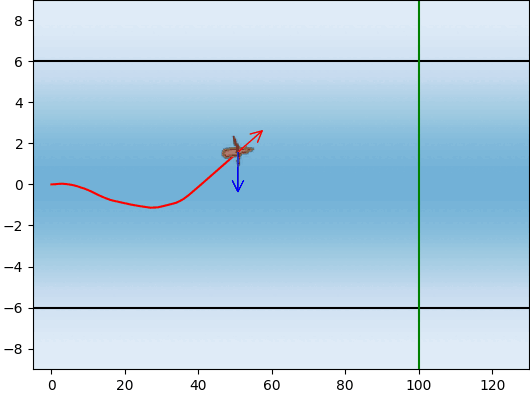
\includegraphics[width=\textwidth]{graphics/boat_frame_example_2.png}
    \centering
    \caption{Visualiserung des Schiff-Agentens während einer überfahrt mit Windeinfluss (Blauer Pfeil) und richtungs Vektor (Roter Pfeil).}
    \label{abb:boat_frame_example_2}
\end{figure}
In Abbildung \ref*{abb:boat_frame_example_2} ist zu erkennen, wie das Schiff eine grüne Ziellinie hat, welche es unbedingt erreichen soll damit eine Episode innerhalb des Reinforcement Learnings erreicht ist. Außerdem ist durch schwarze Linien ein äußerer Bereich von -6 bis 6 gekennzeichnet, welches das Schiff nicht überschreiten soll. Ein überschreiten führt beim Training des Agenten zu einer frühzeitigen beeindigung der Episode. Des weiteren soll eine Störgröße das Schiff beziehungsweise den Agenten bei seiner überfahrt beeinflussen, damit der Agent lernen soll dieses Störgröße automatisch auszugleichen. Die Störgröße in Form von einem Wind im Modell vorhanden sein, der Wind kann dabei aus jeder Richtung wähen und verändert sich mit der Zeit in der Richtung und in der Windstärke. Innerhalb der Abbildung \ref*{abb:boat_frame_example_2} ist der Wind erkennbar an einem kleinen blauen Pfeil am Schiff selbst.\\
Die Modellbildung selbst findet nun statt aus der Perspektive des Schiffs, die tatsächliche Kinematik, sprich die zum Beispiel die Richtung in welche sich das Schiff dann im Environment bewegt wird in einem späteren Schritt dann umgerechnet.
Modelliert wird das Schiff durch drei Bewegungsgleichungen, welche die Kräfte in longitudinaler, transversaler und das Giermoment des Schiffs beschrieben.
\begin{figure}[H]
    \includegraphics[width=0.7\textwidth]{graphics/ship_eoms.pdf}
    \centering
    \caption{Die drei Bewegungsgleichungen des Schiffs.}
    \label{abb:ship_eoms}
\end{figure}

\subsection{Die erste Bewegungsgleichung des Modells} \label{sec:eom1}
Die erste Bewegungsgleichung für die Bewegung in longitudinaler Richtung, setzt sich zusammen aus den folgenden Kräften.
\begin{align}
    F_{Lon} = F_{T} - F_{Rl} + F_{Cl} \label{eq:longitudinal_force}
\end{align}
Der Antrieb des Schiffs wird modelliert durch eine Gleichung, welche abhängig von der Drehgeschwindigkeit der Schiffsschreube einen Schub generiert.
\begin{align}
    F_{T} = K_T(J) \cdot \rho \cdot d^4 \cdot n^2 \cdot (1-t) \label{eq:thrust_force}
\end{align}
wobei,
\begin{enumerate}
    \item[] $\rho = 1$, die Wasserdichte
    \item[] $d = 1$, der Schraubendurchmesser
    \item[] $n$, die Drehzahl des Schaube mit $0 \leq n \leq 30$
    \item[] $t = 0.3$, der Leistungsabzug für die Schraube
\end{enumerate}
das $K_T(J)$ entspricht einer Kennlinie welche individuel für einen gegebenen Schaube per Experimenteller Messung bestimmt wird. Da dies für diese Arbeit jedoch nicht möglich ist, wurde dieses Kurve stattdesen mit einer Sinus-Kurve approximiert. Das $J$ in Gleichung \ref*{eq:thrust_force} der Gleichung, entspricht dem Vorschubsquotient, dieser Wert beschreibt wieviel tatsächlicher Schub von der Schaube aus generiert werden kann abhängig von der momentanen longtiudinalen Geschwindigkeit des Schiffs zur Drehgeschwindigkeit der Schiffschraube.
\begin{align}
    J = \frac{v_l \cdot (1-w)}{n \cdot d} \label{eq:thrust_coeffcient}
\end{align}
wobei,
\begin{enumerate}
    \item[] $v_l$, die longitudinale Geschwindigkeit des Schiffs
    \item[] $w$ = 0.3, Nachlaufströmungs Koeffizient
\end{enumerate}
Der Widerstand, welcher ausgehend vom Wasser auf das Schiff longitudinal wirkt und somit das Schiff auch ausbremst ist definiert als reguläre Widerstandsgleichung abhängig der momentanen Geschwindigkeit des Schiffs.
\begin{align}
    F_{Rl} = \frac{1}{2} \cdot v_l^2 \cdot \rho \cdot c_{Sl} \cdot A_{Sl} \label{eq:front_resistance}
\end{align}
wobei,
\begin{enumerate}
    \item[] $c_{Sl} = 0.31$, der Reibungskoeffient des Schiffs von Vorne
    \item[] $A_{Sl} = 20$, die Fläche des Schiffs von vorne
\end{enumerate}
entspricht. Als weitere Kraftkomponente um das Schiff noch dynamischer zu machen während es eine Kurve zieht, wird außerdem eine Kraft für die Zentripedalkraft definiert innerhalb von $F_C$. Die stimmt nicht ganz mit der realen Definition für die Zentripedalkraft überein, liefert allerdings dennoch gute Ergebnisse und wird somit als annäherung verwendet.
\begin{align}
    F_C = v_t \cdot v_r \cdot (m_{s}+ m_{St})
\end{align}
wobei,
\begin{enumerate}
    \item[] $v_t$, die transversale Geschwindigkeit des Schiffs
    \item[] $m_s$, die Masse des Schiffs
    \item[] $m_{St}$, die Masse des Schiffs in transeversaler Richtung durch Trägheit
    \item[] $v_r$, die Winkelgeschwindigkeit des Schiffs
\end{enumerate}
entsprechen.

\subsection{Die zweite Bewegungsgleichung des Modells} \label{sec:eom2}
Die zweite Bewegungsgleich für die Bewegung des Schiffs in transversaler Richtung, setzt sich zusammen aus den folgenden Kräften.
\begin{align}
    F_{Tra} = F_{Ru} - F_{Rt} + F_{Ct}
\end{align}
Im Vergleich zu der ersten Bewegungsgleichung, gibt es in der zweiten keine Kraft, welche direkt neue Kraft generiert. Die Kräfte, welche sich in in diesem Fall bilden, kommen aus indirekter Abhängigkeit zu dem Schub, welcher in der ersten Kraftgleichung gebildet wird. Die erste Kraft, welche Abhängig vom Schub in der zweiten Bewegungsgleichung gebildet wird, kommt vom Ruder des Schiffs, welches im Winkelbereich von $-\frac{\pi}{3} \leq \alpha \leq \frac{\pi}{3}$ vom Agenten bewegt werden kann. Das $F_{Ru}$ ergibt sich somit zu der folgenden Gleichung, welche auf die bereits verwendetet Widerstandsgleichung basiert. Der Unterschied liegt jedoch darin, dass die Fläche des Ruders als variabel angesehen wird und abhängig vom Rudderwinkel bestimmt wird und das Ruder in diesem Modell nur die Geschwindigkeit in longitudinaler Richtung als Abhängigkeit besitzt.
\begin{align}
    F_{Ru} = \frac{1}{2} \cdot v_l^2 \cdot \rho \cdot c_{Ru} \cdot A_{Ru} \cdot \sin(\alpha) \label{eq:rudder_resistance_long}
\end{align}
Wie bereits in der ersten Bewegungsgleichung wird auch in diesem Fall wieder eine weiterer Widerstandsgleichung verwendet um das Schiff selbst in der transversalen Richtung passiv abzubremsen. Diese Gleichung ist Analog zum longitudinalen Fall, nur das hier eine größere Fläche exisitiert und der Reibungskoeffient als ein Rechteckigefläche gewählt wird und somit gilt das $A_{St} = 90$ und $c_{St} = 2$ gilt.
\begin{align}
    F_{Rt} = \frac{1}{2} \cdot v_l^2 \cdot \rho \cdot c_{St} \cdot A_{St} \label{eq:side_resistance}
\end{align}
Auch die Zentripedalkraft $F_{Ct}$ ist erneut ähnlich wie bereits in der ersten Bewegungsgleichung, nur das in diesem Fall eine Abhängigkeit zur longitudinalen Richtung der Geschwindigkeit besteht. In diesem Fall wird außerdem die Masse ausgehend aus der Trägheit in longitudinaler Richtung verwendet, welche mit $m_{Sl} = 50$ gewählt wurde.
\begin{align}
    F_{Ct} = v_l \cdot v_r \cdot (m_{s}+ m_{Sl})
\end{align}
\subsection{Die dritte Bewegungsgleichung des Modells} \label{sec:eom3}
Die dritte und letzte Bewegungsgleichung, welche in diesem Modell verwendet wird sorgt dafür, dass sich das Schiff drehen kann und verwendet hierfür das Drehmoment welches im Gleichgewicht stehen muss. Die Rotation entsteht dadurch das dass Ruder in einen Winkel gesteuert wird, welcher nicht 0 ist. Ausgebremst werden soll die Rotation durch die Hülle des Schiffs zusammen mit der Fläche des Ruders. Wie stark die Rotationsgeschwindigkeit nun ist, ist abhängig davon wie stark das Ruder eingelengt wird, und außerdem für wie lange es eingelenkt ist. Durch die ausbremsung der Rotationsgeschwindigkeit kommt diese irgendwann in eine equilibrium und das Schiff zieht Kreise. In diesem Fall sollen diese Kräfte auch erneut durch Widerstandsgleichungen approximiert werden.
\begin{align}
    M = M_{Rul} - M_S
\end{align}
Die bereits erwähnte Kraft $M_{Rul}$, welche abhängig von der momentanen longtudinalen Geschwindigkeit ein Drehmoment auf das Schiff durch das Ruder wirkt wird beschrieben durch die folgende Gleichung.
\begin{align}
    M_{Rul} = \frac{1}{2} \cdot v_l^2 \cdot \rho \cdot c_{Ru} \cdot A_{Ru} \cdot \sin(\alpha) \cdot \frac{b}{2}
\end{align}
Erkennbar ist die Widerstandsgleichung, welche durch einen Hebelarm bestehend aus der breite des Schiffs mit $b = 6$ erweitert wurde um einen Drehmoment zu bestimmen.
Der größte Drehmoment, welcher nun ausgehend von der Schiffshülle kommt und gegen den Drehmoment des Ruders wirken soll als ausgleich, soll beschrieben werden durch.
\begin{align}
    M_S = \frac{1}{2} \cdot v_r^2 \cdot \rho \cdot c_{St} \cdot A_{St} \cdot l
\end{align}
Auch hier wurde erneut eine Widerstandsgleichung um einen Hebelarm erweitert, da nun allerdings die ganze Seite des Schiffs betrachtet wird, wurde hier auch die komplette länge des Schiffes verwendet. Wichtig ist an dieser Stelle, das die länge des Schiffs um einiges höher skaliert werden musste, als was sie eigentlich ist. In dieser Arbeit wurde bei dem Drehmoment zum Beispiel $10 \cdot l$ verwendet, da dass Schiff sonst nicht mehr in Ruhelage kommt.

\subsection{Die Kinematik und Umrechnung der Modellinformationen} \label{sec:kinematik}
Da dass Modell aus der Perspektive des Schiffs modelliert ist, wurde ein Subsystem implementiert, welches das Modell in ein neues Koordinatensystem transformiert umso eine einfachere Schnittstelle zum Agenten herzustellen. Die Kinematik dient zum Beispiel dazu, die aktuelle Position des Schiffs im gesamten Environment zu erhalten, oder in welche tatsächliche Richtung es überhaupt ausgerichtet ist. Damit soll es dem Agenten möglich sein ein besseren Oberservationspace bilden zu können.

Der Betrag der Geschwindigkeit gibt sich aus dem Pythagoras der beiden Geschwindigkeitskomponenten $v_x$ und $v_y$.
\begin{align}
    v = \sqrt[2]{v_x^2 + v_y^2}
\end{align}
Die Winkel $\beta$, welcher Beschreibt in welche Richtung das Schiff treibt, wird bestimmt durch
\begin{align}
    \beta = \arccos \left( \frac{v_x}{v_y} \right)
\end{align}
Die tatsächliche Ausrichtung des Schiffs $s_r$ ist lediglich das Integral der momentanen Drehgeschwindigkeit $v_r$
\begin{align}
    s_r = \int_{t}^{t+\Delta t} v_r \, dt
\end{align}
Die nun umtransformierte Position des Schiffs in $x$ und $y$-Position ergibt sich aus
\begin{align}
    s_x = \int_{t}^{t+\Delta t} v \cdot \sin(\beta - s_r) \, dt
\end{align}
\begin{align}
    s_y = \int_{t}^{t+\Delta t} v \cdot \cos(\beta - s_r) \, dt
\end{align}


\section{Einbindung des Modells in Python} \label{sec:simulink_to_py}
Das funktionierende Simulink Modell muss für die verwendung zusammen mit dem Agenten, in Python umgesetzt werden. Damit dies gelingen kann, wurde festgelegt, dass das Ziel sein soll einige Blöcke aus Simulink nachzuahmen umso eine fast identische Funktionalität zuhaben wie sie in Simulink vorliegt. Da innerhalb von Simulink Blöcke verwendet werden, welche verbunden werden durch Kanten und dies in Python nicht möglich ist. Werden innerhalb von Python stattdesen Klassenattribute verwendet um zum Beispiel die gesamt Beschleunigung eines Modells zu definieren. Ein solches Klassenattribute kann damit nun zum Beispiel verwendet werden um einen Feedback-Loop zu modellieren, wie es in Simulink mithilfe von zurücklaufenden Kanten gemacht wird. Die Integratoren welche in Simulink mit das Kernstück und eine der wichtigesten Blockarten ist, wurde in Python nachgebaut innerhalb einer Integrator Klasse. Die Klasse wurde so implementiert, dass für jeden Integratorblock, welcher aus einem Simulink Modell übernommen werden soll, ein Integrator Object definiert wird. Dies könnte dann folgend aussehen in einem Quellcode Beispiel.
\begin{lstlisting}[language=Python]
a_integrator = Integrator()
v_integrator = Integrator(initial_value=h_0)
\end{lstlisting}
Hier in diesem Quellcode Ausschnitt ist zu sehen, dass ein Integrator für jeweils die Beschleunigung und Geschwindigkeit eines Modells definiert sind. Zudem kommt hinzu, dass für den Integrator von Geschwindigkeit auf Position ein Initialwert gesetzt wurde von $h_0$. Es wurde außerdem aus Simulink die Integrator Fuktion nachgebaut um ein oberes und unteres Limit für die Integration zu setzen, auch diese würde als Argument übergeben werden können bei einem jeweiligen Integrator.\\
Die Integratoren selbst funktionieren nun so, dass sie eine eigene Klassenmethode besitzen, welche als Argument ein beliebiges Signal erwartet. Dieses Signal würde etwa der gesamt Beschleunigung oder Geschwindigkeit eines Modells entsprechen, hier in diesem Fall würden zum Beispiel also die Klassenattribute sein, welche bereits erwähnt wurden. Das eingehende Signal wird dann integriert nach folgender Formel.
\begin{align*}
    s' = \int_{t}^{t+dt} s \, dx
\end{align*}
Die Signal $s$ wird gesehen als eine Konstante, welche integriert wird vom Zeitschritt $t$ bis $t + dt$, wobei das $dt$ hier vorschreibt wie groß der Integrationschritt letztendlich sein soll. Innerhalb dieser Arbeit wurde $dt = 0.1$ gewählt, da es die ausreichende größe bietet um das gewählte Modell zu simulieren ohne großem Genauigkeitsverlust.
\newpage
\subsection{Testen des Integrators anhand eines einfachen Beispiels} \label{sec:integrator_test}
Um die Integrator Klasse in Python zu testen bevor sie für das richtige Schiffmodell verwendet wird, wurde ein einfaches Modell erstellt, in welchem ein Fallschirmspringer in einer bestimmten Höhe abspringt und irgendwann den Fallschirm öffnet und verlangsamt auf dem Boden ankommt. In diesem Fallschirm Modell wurde der Fallschirm so modelliert, das er ab eine Höhe von 1500 aufgeht und damit seine Fläche deutlich größer wird. Diese größere Fläche spiegelt sich dann wieder in der reduzierten Fallgeschwindigkeit des Fallschirmspringers. Beschrieben werden kann das Fallschirmmodell durch die folgende Kraftgleichung.
\begin{align*}
    F = -F_G + F_W
\end{align*}

Wobei das $F_G$ der Kraft entspricht, welche sich aus der Fallbeschleunigung $g$ und der Masse des Fallschirmspringers zusammensetzt. $F_W$ entspricht dem Wind Widerstand, welcher abhängig von der Fläche des Fallschirmspringers beziehungsweise des Fallschirms sich ändert. Sie wird modelliert durch die folgende Gleichung für den Widerstand.

\begin{align*}
    F_W = \frac{1}{2} \cdot v^2 \cdot \rho \cdot c \cdot A
\end{align*}
wobei hier $A$ die Fläche des Fallschirmspringers selbst oder des Fallschirmspringers mit Fallschirm ist. Selbes gilt auch für den Reibungskoeffient $c$.

In Simulink ergibt sich das gesamte Modell zu der folgenden Struktur, in welcher die einzelnen Kraftkomponenten und besonderen Funktionen wie das abbrechen des Modells sobald die Höhe 0 erreicht ist, Farblich hinterlegt sind.

\begin{figure}[H]
    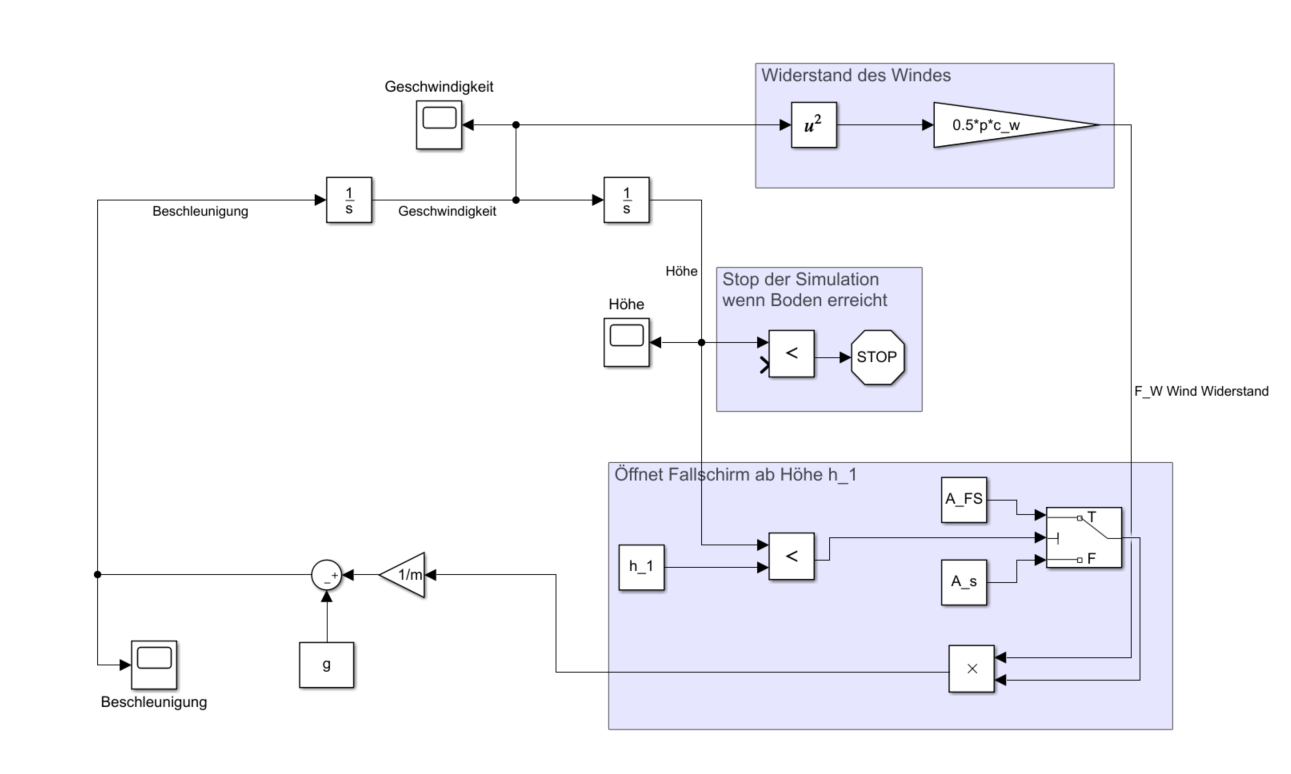
\includegraphics[width=\textwidth]{graphics/parachute_simulink.png}
    \centering
    \caption{Das Fallschirm Modell in Simulink}
    \label{abb:parachute_simulink}
\end{figure}

Das gleiche Modell nun modelliert in Python ergibt sich zu folgenden Quellcode.

\begin{lstlisting}[language=Python]
from control_theory.control_blocks import Integrator

if __name__ == '__main__':
    # Define constants
    h_0 = 3000
    h_1 = 1500
    A_s = 0.5
    A_FS = 25
    m = 85
    c_w = 1.3
    p = 1.2
    g = 9.81
    t, t_max, dt = 0, 500, 0.1

    # Define integrator objects
    a_integrator = Integrator()
    v_integrator = Integrator(initial_value=h_0)

    total_a = 0
    while t <= t_max:
        # Integrate acceleration and velocity
        total_a -= g
        v = a_integrator.integrate_signal(total_a)
        s = v_integrator.integrate_signal(v)

        # Stop if ground reached
        if s < 0:
            break

        # Wind resistance
        if s < h_1:
            F_w = v**2 * 0.5 * p * c_w * A_FS
        else:
            F_w = v**2 * 0.5 * p * c_w * A_s
        # Turn force into acceleration
        total_a = F_w / m

        t += dt

\end{lstlisting}

Zusehen ist, dass das Modell in Python angetrieben wird durch eine $while$-Schleife, welche terminiert sobald das $t_{max}$ erreicht ist. Innerhalb der $while$-Schleife wird dafür die Laufvariabel $t$ inkrementiert durch ein zuvor festgelegtes $dt$, welches in den zuvor definierten Integralen dem $\Delta t$ und somit der Integrationsschrittgröße entspricht. Konstanten wurden außerhalb der $while$-Schleife definiert zusammen mit einem $total\_a$, welches die gesamt Beschleunigung des Modells beschreibt. Die Integratoren werden nun innerhalb der $while$-Schleife verwendet um die gesamt Beschleunigung in eine Geschwindigkeit und anschließend in die Höhe des Fallschirmspringers zu integrieren. Basierend auf diesen Methodenrückgaben können dann veränderungen an den Signalen vorgenommen werden um zum Beispiel das $F_W$ abhängig von der Höhe zu bestimmen.\\
Ein direkter Vergleich der Ergebnisse unter verwendung der gleichen konstanten bei den beiden Modellvarianten in Python und Simulink zeigt dann auch gleich, dass die Integratoren und der Ansatz für die Modellierung in Python korrekt sind. Anzumerken ist jedoch, dass die Zeitaxen sich bei den beiden Plots ein wenig unterscheiden, dies ist jedoch darauf zurückzuführen, wie Simulink die Zeitschritte definiert und wie sie im Python Modell definiert sind. In diesem Fall ist es einfach nur eine unterschiedliche Skalierung.
\begin{figure}[H]
    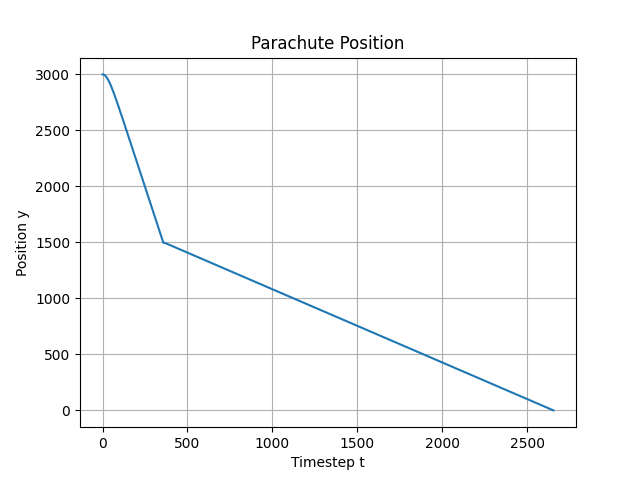
\includegraphics[width=\textwidth]{graphics/python_parachute_s_plot.png}
    \centering
    \caption{Plot der Höhe des Fallschirmspringers gegen die Zeit im Python Modell}
    \label{fig:python_parachute_s_plot}
\end{figure}

\begin{figure}[H]
    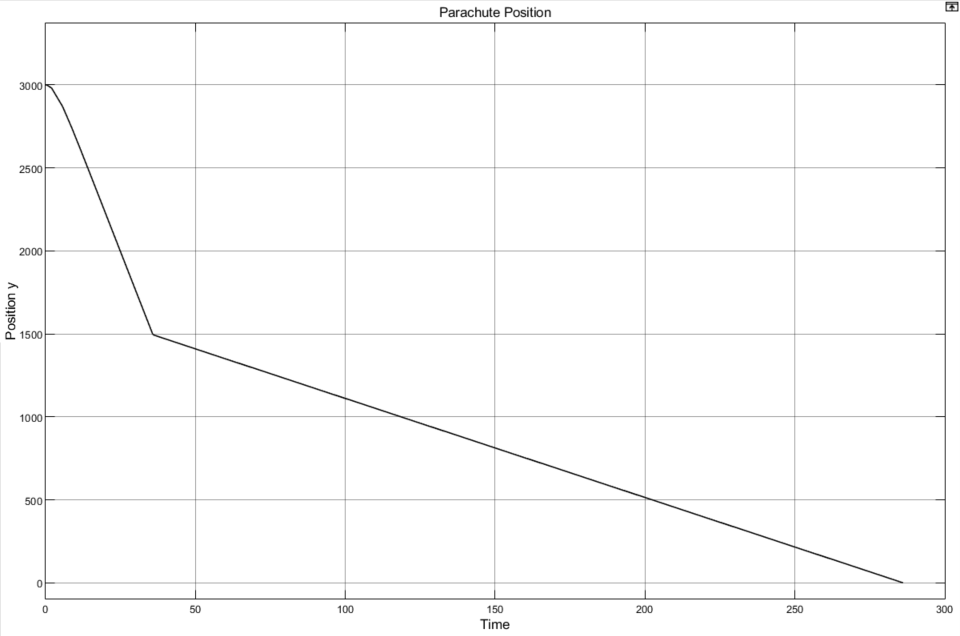
\includegraphics[width=\textwidth]{graphics/simulink_parachute_s_plot.png}
    \centering
    \caption{Plot der Höhe des Fallschirmspringers gegen die Zeit im Simulink Modell}
    \label{fig:simulink_parachute_s_plot}
\end{figure}

\newpage
\subsection{Aufbau des Schiffmodells} \label{sec:aufbau_schiffsmodell}

\chapter{Ergebnisse} \label{sec:ergebnisse}

\chapter{Diskussion} \label{sec:diskussion}

\chapter{Zusammenfassung und Ausblick} \label{sec:zsmfassung_ausblick}

\end{document}